\chapter{Présentation de l’entreprise}

\section{Historique}

INTERFACE est un groupe multinational créé en 1994 avec pour objet l’application des technologies de l’information et de la communication aux problématiques métiers. Le groupe s’est progressivement affirmé comme architecte d’infrastructures, éditeur de solutions logicielles, conseil en stratégie, en innovation et en technologies, assumant ainsi pleinement une approche métier singulière, faite d’anticipation des contraintes fonctionnelles. \\
La création du pôle Consulting a marqué un virage majeur du développement de notre groupe, avec la création en fin 2014 d’InterAsys Conseils, cabinet spécialisé dans le Conseil, le Management et l’Organisation. Aujourd’hui présents dans une dizaine de pays européens et africains, INTERFACE démontre au quotidien la capacité à accompagner les organisations publiques et privées dans le choix des technologies adaptées à leur métier, et l’alignement maîtrisé de leurs systèmes d’information à leur stratégie de développement.

\section{Fiche d'informations}

\begin{table}[H]
    \centering
    \caption{Fiche d'informations sur INTERFACE}
    \begin{tabular}[t]{|p{7.5cm}|p{7.5cm}|} 
        \hline\hline
        \textbf{Nom ou raison sociale } & INTERFACE SA\\
        \hline
        \textbf{Adresse } & 1251, Boulevard de la BESSEKE ; BP : 12423 Douala \\
        \hline
        \textbf{No du contribuable  } & M0794000000978Y \\
        \hline
        \textbf{Téléphone  } & (237) 33 42 57 16  Fax. (237) 33 42 57 17   \\
        \hline
        \textbf{Email  } & interface@interfacesa.com \\
        \hline
        \textbf{Registre de Commerce de  } & Douala \\
        \hline
        \textbf{Sous le numéro  } & 013074 \\
        \hline
        \textbf{Date d’enregistrement  } & 05/07/1994  \\
        \hline
        \textbf{Capital  } & 656 000 000 F.CFA \\
        \hline
        \textbf{Effectif du personnel permanent } & 300 Salariés et Consultants permanents \\
        \hline
        \textbf{Filiales } & Interface France, Interface Congo, Interface RCA, Interface Tchad, Interface RDC, Interface Gabon, Interface RSA, Logis SA, InterAsys Conseils  \\
        \hline
        \textbf{Succursales } & Yaoundé, Douala, Pointe-Noire, Lagos, Lubumbashi \\
        \hline
        \textbf{Représentations commerciales } & Représentations commerciales	Luanda, Niamey, Cotonou, Malabo, Maputo, Abidjan \\
        \hline
        \textbf{Centre d’Expertise et de Compétence du groupe INTERFACE (CECI) } & France : 5, Avenue de la Mare, 95310, Saint-Ouen l’Aumône \\
        \hline
        \textbf{Centre de Recherche – Développement du groupe INTERFACE (CRDI) } & République Sud-Africaine : 11, Galaxy Avenue, Linbro Business Park, Sandton, Johannesburg \\
        \hline
    \end{tabular}
    \label{tab:infostab}
\end{table}


\begin{table}[H]
    \centering
    \begin{tabular}[t]{|p{7.5cm}|p{7.5cm}|} 
        \hline
        \textbf{Centre de Formation Qualifiante et Certifiante du groupe INTERFACE (Training Center) } & 
            Cameroun : 1251, Boulevard de la Besseke, Douala, 
            France : 5, Avenue de la Mare, 95310, Saint-Ouen l’Aumône
         \\
        \hline\hline
    \end{tabular}
\end{table}


\section{Organisation}
INTERFACE SA est structurée en 6 pôles d’excellence, dirigés par des experts hautement qualifiés 
\paragraph{Le pôle Consulting :} assiste les clients dans la maîtrise d’ouvrage des projets IT stratégiques. Il intègre : (i) le CECI (Centre d’Expertise et de Compétences d’INTERFACE), véritable Skills Center (ii) et le Training Center (Centre de formation qualifiante et certifiante), pour l’accompagnement nécessaire à la montée en compétences de nos clients et partenaires. Pour se déployer, ce pôle s’appuie désormais sur les capacités et compétences offertes par InterAsys Conseils. 
\paragraph{Le pole Software Engineering :} éditeur et intégrateur d’une solution ERP verticale orientée métier, baptisée my e-Sésame ainsi que  d’autres applications informatiques horizontales développées au forfait. Il intègre le CRDI (Centre de Recherche et de développement d’Interface), dont la localisation en Afrique du Sud favorise de nombreux échanges entre nos experts et les communautés informatiques de l’Inde et de l’Île Maurice.

\paragraph{Le pôle Systèmes et Infrastructures :} Architecte et Infogérant d’infrastructures de stockage, serveurs, réseaux et télécoms basées sur les technologies les plus récentes (Ibm, Hp, Cisco, VMware, Oracle, Linux, Grandstream…).

\paragraph{Le pôle Business Information Management :} spécialiste des technologies de gestion de contenu d’entreprise, de gestion électronique des documents (GED), d’optimisation du cycle documentaire et gestion des bases de données Oracle et Sql Server.

\paragraph{Le pôle Banking Solutions :} dédié aux solutions spécifiques au secteur financier : monétique, cash cycle management, dématérialisation des services financiers, éditique bancaire, core banking et BPO.

\paragraph{Le pôle Distribution :} grossiste africain de plusieurs constructeurs (Ibm, Lexmark, Hp, Lenovo, Dell, Nitram, Epson, Canon, Etc.). Depuis 2010, ce pôle s’appuie sur les capacités et compétences offertes par LOGIS SA, filiale du groupe INTERFACE, spécialisée dans le transport, la logistique, le transit  et la centrale d’achats.

INTERFACE est gouverné par un Comité de Direction (CODIR) constitué de :
\begin{itemize}
    \item \textbf{Tatiana OBONO}, Directeur Général Adjoint du groupe INTERFACE et Présidente du CODIR
    \item \textbf{Jules Daniel OWONA}, Directeur d’INTERFACE Yaoundé
    \item \textbf{Gordon BALL}, Managing Director of INTERFACE SYSTEMS MANAGEMENT Ltd (RSA) and of the Center for Research and Development (CRDI)
    \item \textbf{François Xavier TARI}, Directeur d’INTERFACE France et du Centre d’Expertise et de Compétence (CECI)  
    
\end{itemize}




\section{Organigramme fonctionnel}
\begin{figure}[H]
    \centering
    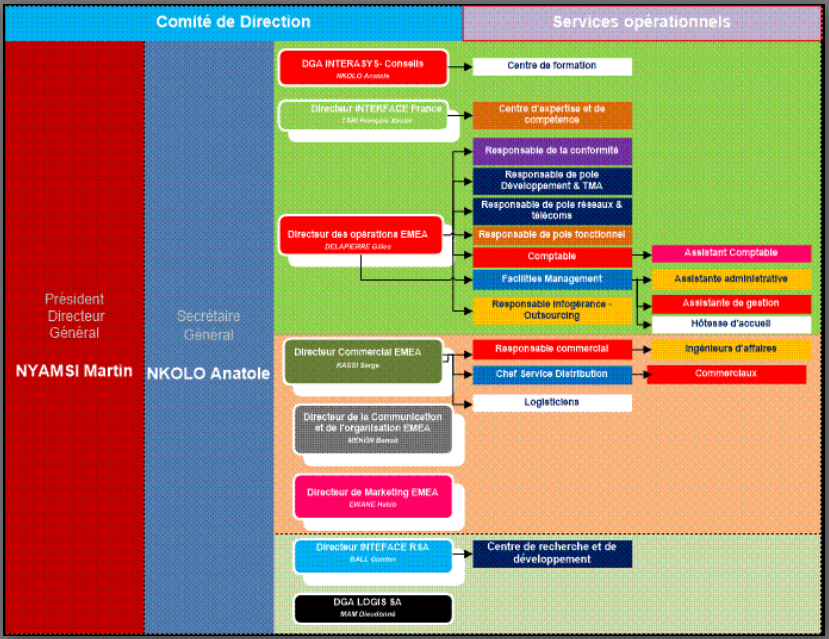
\includegraphics[width=\textwidth]{organigramme}
    \caption{Organigramme fonctionnel d'INTERFACE SA}
    \label{fig:organigramme}
\end{figure}
%\section{Schéma de fonctionnement}

\section{Plan de localisation}
\begin{figure}[H]
    \centering
    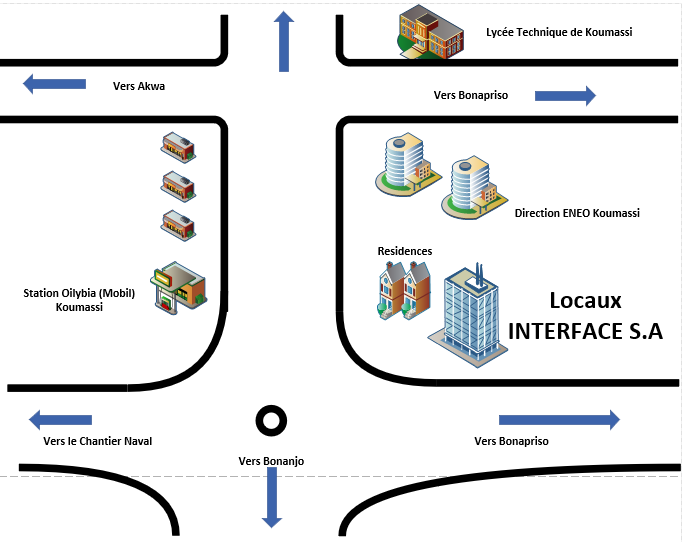
\includegraphics[width=\textwidth]{localisation}
    \caption{Plan de localisation d'INTERFACE SA}
    \label{fig:localisation}
\end{figure}
\section{Métiers}
INTERFACE associe 4 métiers complémentaires pour mieux répondre aux besoins de ses clients, et ce, dans le but de les accompagner sur l’ensemble de la chaîne de valeur.
\begin{itemize}
    \item Conseil en stratégie, en innovation et en technologies numériques ;
    \item Architecte et Infogérant d’infrastructures IT ;
    \item Editeur de solutions logicielles ; 
    \item Distributeur de  marques. 
\end{itemize}

\section{Capacités}
Afin de répondre à des projets de plus en plus complexes et aux exigences des clients de plus en plus importants, notamment les grands comptes, INTERFACE a noué des partenariats garants de la maîtrise technique, commerciale et financière de nos prestations et solutions. 
\paragraph{Au plan organisationnel et technique}, la localisation en France de la Direction du Développement International en charge de la gestion des Alliances et Partenariats, du Centre d’Expertise et de Compétence (CECI), du Training Center pour les ressortissants de l’Europe, des Amériques et de l’Asie, ainsi que la filialisation dans LOGIS SA de nos activités de transport, logistique, transit  et centrale d’achats, facilitent :
\begin{itemize}
    \item La conclusion de partenariats win-win avec des leaders mondiaux tels que Ibm, Capgemini, Lexmark, Lenovo, Supinfo, Oracle, Cisco, Microsoft, Loglogic, Wincor/Nixdorf… ;
    \item La montée en compétences du personnel et des consultants.
\end{itemize}

\paragraph{Au plan financier}, la capacité d’INTERFACE à réaliser avec sérénité les missions qui lui sont confiées est garantie et soutenue par la confiance que lui font ses partenaires financiers en l’occurrence :
\begin{itemize}
    \item \textbf{Au Cameroun :}
    \begin{itemize}
        \item BICEC (Banque International du Cameroun pour l’Epargne et le Crédit),
        \item SGBC (Société Générale de Banque au Cameroun),
        \item CBC (Commercial Bank of Cameroon).
    \end{itemize}
    \item \textbf{En France :} Société Générale.
    \item \textbf{En Afrique du Sud :} ABSA Bank.
    \item \textbf{Au Congo Brazzaville :} CBI Congo
\end{itemize}

En plus des ressources financières mobilisables auprès des financiers précités, d’autres partenaires tels que Lexmark, Capgemini Consulting, Supinfo…, sont disposés à mobiliser pour le compte des projets confiés à INTERFACE, tout ou partie des moyens matériels, logiciels et humains souhaités.

\section{Perspectives}
Pour aborder l’avenir avec sérénité et professionnalisme, INTERFACE s’appuie sur deux principaux leviers d’action :
\begin{itemize}
    \item \textbf{Expansion et Consolidation :}INTERFACE envisage dans un proche avenir la création de nouvelles entités en vue de répondre de manière satisfaisante aux exigences de qualité, de coût et de délai de notre clientèle
    \item \textbf{Valorisation du pôle d’excellence technologique :} INTERFACE entend renforcer et développer de nouveaux partenariats stratégiques avec des leaders mondiaux dans le domaine des TIC et de l’économie numérique, afin d’offrir à sa clientèle une gamme complète et variée de solutions intelligentes et innovantes.
\end{itemize}  


